\documentclass[conference]{IEEEtran}
\IEEEoverridecommandlockouts%The preceding line is only needed to identify funding in the first footnote. If that is unneeded, please comment it out.

\usepackage[utf8]{inputenc}
\usepackage{cite}
\usepackage{amsmath,amssymb,amsfonts}
\usepackage{algorithmic}
\usepackage{graphicx}
\usepackage{textcomp}
\usepackage{xcolor}
\usepackage{lipsum}


\def\BibTeX{{\rm B\kern-.05em{\sc i\kern-.025em b}\kern-.08em
    T\kern-.1667em\lower.7ex\hbox{E}\kern-.125emX}}

%Para justificar sin cortar palabras
\tolerance=1
\emergencystretch=\maxdimen
\hyphenpenalty=10000
\hbadness=10000

\def\shadowLine{\vspace{3mm}}
\def\shadowMath{\\[3mm]}

%-------------------------------------------------------------------------------
%	BEGIN DOCUMENT
%-------------------------------------------------------------------------------
\begin{document}

%-------------------------------------------------------------------------------
%	DOCUMENT INFORMATION
%-------------------------------------------------------------------------------
\title{Práctica 1 - MTF del ojo humano}


%-------------------------------------------------------------------------------
%	AUTHORS
%-------------------------------------------------------------------------------
\author{
\IEEEauthorblockN{Daniel Torres Robledo}
\IEEEauthorblockA{\textit{shadow.cat6333@gmail.com}}
\and
\IEEEauthorblockN{Andrés Fuentes Hernández}
\IEEEauthorblockA{\textit{andres7233@hotmail.com}}

}

\maketitle


%-------------------------------------------------------------------------------
%	ABSTRACT
%-------------------------------------------------------------------------------
\begin{abstract}
En este documento se describen las aplicaciones de la \textit{MTF}, el cálculo de ecuaciones para generarla, su implementación en \textit{python}, así como experimentos utilizando este estímulo con diferentes personas a distintas distancias, que para obtener medidas invariantes a la distancia de observación, el cálculo de esta frecuencia será expresado en ciclos/grado.
\end{abstract}

\begin{IEEEkeywords}
MTF, SVH, python, sinusoidal modulada, experimentos, invariantes
\end{IEEEkeywords}


%-------------------------------------------------------------------------------
%	SECTION 1
%-------------------------------------------------------------------------------
\section{\textit{Objetivo}}


\begin{itemize}
\item Encontrar la \textit{MTF} del ojo experimentalmente.
\item Encontrar la frecuencia de máxima sensibilidad del ojo humano.
\item Generar los cálculos necesarios para obtener la función sinusoidal en frecuencia y amplitud.
\item Desplegar el estímulo visual sinusoidal modulada.
\end{itemize}


%-------------------------------------------------------------------------------
%	SECTION 1
%-------------------------------------------------------------------------------
\section{\textit{Introducción}}

La \textit{MTF} (\textit{Modulation Transfer Function}) o función de transferencia de modulación se ha convertido en una herramienta muy utilizada para especificar el rendimiento y la resolución de toda clase de sistemas ópticos y de visión, que van desde lentes, cintas magnéticas y películas hasta telescopios, la atmósfera y el ojo humano.

La \textit{MTF} es usada para caracterizar sistemas lineales e invariantes en el espacio, sin embargo, a pesar de que el Sistema Visual Humano (SVH) no cumple con estas dos propiedades, la \textit{MTF} se ha utilizado para caracterizarlo bajo condiciones de iluminación controladas.

La \textit{MTF} también puede interpretarse como la capacidad de un sistema óptico para percibir contraste, es decir, la capacidad de resolver o diferenciar líneas a una determinada frecuencia espacial.

Para entender de manera simplificada el concepto de frecuencia espacial, hay que notar que las frecuencias espaciales bajas equivalen a repeticiones de patrones muy separados espacialmente (por ejemplo, líneas muy separadas) y que las altas equivalen a repeticiones más compactas.

Hay que considerar que todo sistema de visión tiene un límite superior a partir del cual ya no le es posible distinguir más detalles. Este límite está directamente relacionado con la frecuencia de \textit{Nyquist}\cite{p4}. En los estudios de sensibilidad del \textit{SVH} a base de experimentación psico-física, se ha encontrado que su \textit{MTF} consiste en una función del tipo paso-banda con un pico o frecuencia espacial máxima en el rango de 2 a 6 ciclos por grado\cite{p1}\cite{p2}.

En esta practica se examinará la sensibilidad del \textit{SVH} a distintas frecuencias espaciales; la idea general de crear un patrón de sinusoidales, cuya frecuencia aumenta en el eje horizontal y el contraste en el eje vertical. La envolvente del patrón visibles generalmente muestra un comportamiento similar a la curva de la \textit{MTF}.

Comprobaremos que dicho pico, que representa la frecuencia máxima de sensibilidad del ojo humano se moverá conforme el observador se aleja o acerca del estímulo. Para obtener una medición invariante a la distancia de observación, el cálculo de esta frecuencia de observación debe ser expresado en ciclos/grado.


%-------------------------------------------------------------------------------
%	SECTION 1
%-------------------------------------------------------------------------------
\section{\textit{Desarrollo}}

En esta sección se muestra el cálculo para obtener las constantes de la función sinusoidal modulada en frecuencia y en amplitud.

Sea la función $I$, que dará los valores de cada pixel de la imagen:

$I(n,m) = g(n)\cdot \sin(2\pi\cdot f(m))$

$h = altura\ de\ la\ imagen$

$w =  ancho\ de\ la\ imagen$

Sea $g$ la función de contraste, donde ses necesario encontrar las constantes $c,d$:

$g(n)=d\cdot e^{-c\cdot n}$

Para el eje horizontal, utilizaremos $f$:

$f(m) = a\cdot e^{b\cdot x}$

Por lo que la frecuencia instantánea esta definida como la derivada de $f$:

$f'(m) = a\cdot b\cdot e^{b\cdot x}$

Es necesario encontrar las constantes $a,b$ tal que $f'(w) = 1/2$ para obtener la frecuencia máxima , y $f'(0) = 1/w$ para encontrar la frecuencia mínima, en $ciclos/segundo$

$1)f'(0) = a\cdot b\cdot e^{b\cdot 0} = a\cdot b \cdot 1= a\cdot b = 1/w$

$2)f'(w) = a\cdot b\cdot e^{b\cdot w} = 1/2$

Para encontrar $b$, sustituir $1\ en\ 2$:

$(1/w)\cdot e^{b\cdot w} = 1/2$

\shadowLine
$e^{b\cdot w} = w/2$

\shadowLine
$ln(e^{b\cdot w}) = ln(w/2)$

\shadowLine
$b\cdot w\cdot ln(e) = ln(w/2)$

\shadowLine
$b = \displaystyle\frac{ln(w/2)}{w\cdot ln(e)}  $

\shadowLine
$b = \displaystyle\frac{ln(w/2)}{w\cdot ln(e)}  $

\shadowLine
$b = \displaystyle\frac{ln(w/2)}{w}  $

Por lo que para encontrar $a$ sustituimos $b$ en $1)$

$a\cdot b = 1/w$

\shadowLine
$a = \displaystyle\frac{1}{b\cdot w}$

Por lo tanto ya tenemos los valores de $a, b$:

$a = \displaystyle\frac{1}{b\cdot w}$

\shadowLine
$b = \displaystyle\frac{ln(w/2)}{w}$

Para encontrar las constantes $c,d$ de $g(n)$ :

\shadowLine
$g(n)=d\cdot e^{-c\cdot n}$

Donde $\epsilon>0$.

\shadowLine
$1)g(0)=d\cdot e^{-c\cdot 0} = d = \epsilon$

\shadowLine
$2)g(h)=d\cdot e^{-c\cdot h} = 1$

Para encontrar $c$, sustituimos 1 en 2:

$\epsilon\cdot e^{-c\cdot h}=1$

\shadowLine
$ln(\epsilon\cdot e^{-c\cdot h})=ln(1)$

\shadowLine
$ln(\epsilon) + ln(e^{-c\cdot h})=0$

\shadowLine
$-c\cdot h\cdot ln(e)=0$

\shadowLine
$c = \displaystyle\frac{ln(\epsilon)}{h}$

Por lo tanto, para $\epsilon>0$, en este caso utilizaremos $\epsilon = 0.02$:

$d = \epsilon = 0.02$

\shadowLine
$c = \displaystyle\frac{ln(\epsilon)}{h}$

\shadowLine
A continuación se muestra el estímulo \textit{MTF} utilizando dichas constantes:

\begin{figure}[htbp]
\centerline{
\includegraphics[width=80mm]{code/mtf}}
\caption{Estímulo visual (sinusoidal modulada).}
\label{mtf}
\end{figure}

Para calcular los valores que se reportarán en los resultados son:

$X:$ coordenada x donde se encontró experimentalmente el punto más alto visible por el usuario.

$\phi=f'(x)= a\cdot b\cdot e^{b\cdot x}$: Qué es la frecuencia instantánea evaluada en $x$, que son ciclo/pixel.

$dd = screensize/w$: Es la distancia entre dos pixels, que es la medida de la imagen en centímetros entre la cantidad de pixels.

$\alpha= \tan^{-1}(dd/distancia)\cdot (180/\pi)$: Resultado en grados/pixels, el valor de distancia es la distancia a la que se encuentra el observador en centímetros.

\shadowLine
$f=\displaystyle\frac{\phi}{\alpha}$: Frecuencia de observación en ciclos/grado


%-------------------------------------------------------------------------------
%	SECTION 1
%-------------------------------------------------------------------------------
\section{\textit{Resultados}}

Para este experimento, se utilizó el estímulo visual \textit{MTF} descrito en la sección de Desarrollo, el cual fue mostrado a tres diferentes personas a las distancias de $30cm,\ 60cm\ y\ 100cm$, en donde fueron calculados para cada distancia los valores de $x,\ \phi,\ \alpha$ y frecuencia de observación $f$. La descripción de estas ecuaciones también se encuentra en el apartado de Desarrollo.

En este experimento se utilizaron las siguientes constantes:
\begin{itemize}
\item $height = 768$: pixels de altura de la imagen
\item $width = 768$: pixels de longitud de la imagen
\item $screensize=13cm$ medida de la imagen en centímetros
\item $distancia\in [30cm,60cm,100cm]$: distancias en centímetros a las que se encuentra el usuario
\item $\epsilon=0.01$: constante para calcular el contraste.
\end{itemize}

\begin{figure}[htbp]
\centering

\begin{tabular}{c|c|c|c|}
	 & $D_1=30cm$ & $D_2=60cm$ & $D_3=100 cm$\\
	\hline
	$X$ & 513 & 430 & 359\\
	\hline
	$\phi'$ & 0.088 & 0.045 & 0.025\\
	\hline
	$\alpha$ & 0.034 & 0.017 & 0.010\\
	\hline
	$f$ & 2.569 & 2.623 & 2.460\\
	\hline
\end{tabular}

\caption{Tabla de resultados, experimento sin lentes y en morado resultados con lentes 1.1.}
\label{res1.1}
\end{figure}


\begin{figure}[htbp]
\centering

\begin{tabular}{c|c|c|c|}
	 & $D_1=30cm$ & $D_2=60cm$ & $D_3=100 cm$\\
	\hline
	$X$ & 627 & 541 & 475\\
	\hline
	$\phi'$ & 0.221 & 0.110 & 0.064\\
	\hline
	$\alpha$ & 0.034 & 0.017 & 0.010\\
	\hline
	$f$ & 6.469 & 6.446 & 6.295\\
	\hline
\end{tabular}
\caption{Tabla de resultados, experimento sin lentes y en morado resultados con lentes 1.2.}
\label{res1.2}
\end{figure}

\begin{figure}[htbp]
\centering

\begin{tabular}{c|c|c|c|}
	 & $D_1=30cm$ & $D_2=60cm$ & $D_3=100 cm$\\
	\hline
	$X$ & 498 & 418 & 358\\
	\hline
	$\phi'$ & 0.078 & 0.041 & 0.025\\
	\hline
	$\alpha$ & 0.034 & 0.017 & 0.010\\
	\hline
	$f$ & 2.275 & 2.380 & 2.440\\
	\hline

\end{tabular}

\caption{Tabla de resultados, experimento 1.3.}
\label{res1.3}
\end{figure}



%-------------------------------------------------------------------------------
%	SECTION 1
%-------------------------------------------------------------------------------
\section{\textit{Conclusiones}}

Se puede observar como el valor de $x$ se mueve a la izquierda conforme se aleja el usuario de la imagen., sin embargo el valor de la frecuencia de observación $f$, en las figuras \ref{res1.1}, \ref{res1.2} y \ref{res1.3} se mantiene aproximadamente igual, este error puede ser en parte por la acción del usuario al dar \textit{click} sobre la imagen y mover el cursor una cierta cantidad de pixels.

Por lo que se cumplió la hipótesis de tener los ciclos/grado constantes, a pesar de la distancia a la que se encuentra el observador.

Todas las pruebas fueron realizadas con el mismo nivel de brillo de la pantalla del dispositivo.

%-------------------------------------------------------------------------------
%	SECTION 1
%-------------------------------------------------------------------------------
\section{\textit{Código fuente}}

A continuación se muestra la implementación de las ecuaciones mostradas en el Desarrollo para calcular el estímulo visual y los valores reportados en los resultados de $x,\ \phi,\ \alpha$ y frecuencia de observación $f$.

Es posible modificar las constates referentes al tamaño de la imagen, la medida en centímetros de ésta, y la distancia a la que se encuentra el usuario en centímetros, esto en las variables definidas en el \textit{main} del programa.

Este programa permite al usuario dar \textit{click} sobre la imagen para tener el valor de la coordenada en $x$, así como los valores reportados en la tabla de resultados calculados de manera automática.

\begin{figure}[htbp]
\centerline{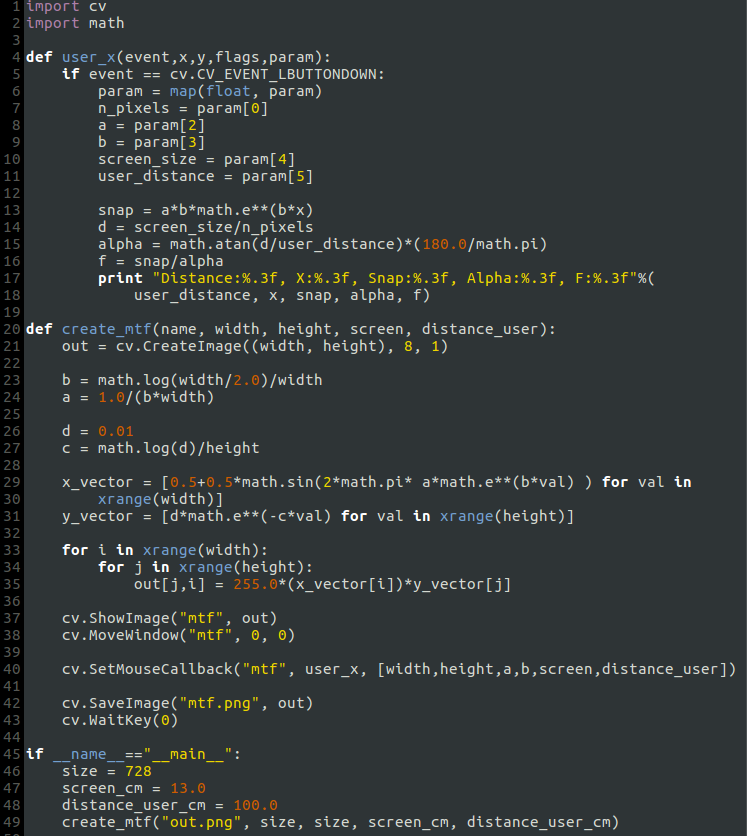
\includegraphics[width=80mm]{code/code1}}
\caption{Código utilizado para la implementación en \textit{python}.}
\label{code1}
\end{figure}

Para la implementación, la función sinusoidal de multiplicó por $0.5$ y se sumó $0.5$ para ajustar los valores al rango  $[0,1]$, ya que estaban en $[-1,1]$.


%-------------------------------------------------------------------------------
%	BIBLIOGRAPHY
%-------------------------------------------------------------------------------
\begin{thebibliography}{00}
\bibitem{p1} Pratt, W. k., Digital Image Processing, John Wiley \& Sons Inc, 2001.

\bibitem{p2} Levine, M.D., Vision in man and machine, McGraw-Hill, 1985.

\bibitem{p3} Norman Koren, \textit{Resolution and MTF curves in scanners and sharpening}. Avalible at \textit{http://www.normankoren.com/Tutorials/MTF2.html}. [Accessed Agosto 31, 2019]

\bibitem{p4} Norman Koren, \textit{Nyquist frequency}. Avalible at \textit{https://en.wikipedia.org/wiki/Nyquist\_frequency}. [Accessed Agosto 31, 2019]
\end{thebibliography}







%-------------------------------------------------------------------------------
%	END DOCUMENT
%-------------------------------------------------------------------------------
\end{document}